\documentclass[12pt,titlepage]{extarticle}
% Document Layout and Font
\usepackage{subfiles}
\usepackage[margin=2cm, headheight=15pt]{geometry}
\usepackage{fancyhdr}
\usepackage{enumitem}	
\usepackage{wrapfig}
\usepackage{float}
\usepackage{multicol}

\usepackage[p,osf]{scholax}

\renewcommand*\contentsname{Table of Contents}
\renewcommand{\headrulewidth}{0pt}
\pagestyle{fancy}
\fancyhf{}
\fancyfoot[R]{$\thepage$}
\setlength{\parindent}{0cm}
\setlength{\headheight}{17pt}
\hfuzz=9pt

% Figures
\usepackage{svg}

% Utility Management
\usepackage{color}
\usepackage{colortbl}
\usepackage{xcolor}
\usepackage{xpatch}
\usepackage{xparse}

\definecolor{gBlue}{HTML}{7daea3}
\definecolor{gOrange}{HTML}{e78a4e}
\definecolor{gGreen}{HTML}{a9b665}
\definecolor{gPurple}{HTML}{d3869b}

\definecolor{links}{HTML}{1c73a5}
\definecolor{bar}{HTML}{584AA8}

% Math Packages
\usepackage{mathtools, amsmath, amsthm, thmtools, amssymb, physics}
\usepackage[scaled=1.075,ncf,vvarbb]{newtxmath}

\newcommand\B{\mathbb{C}}
\newcommand\C{\mathbb{C}}
\newcommand\R{\mathbb{R}}
\newcommand\Q{\mathbb{Q}}
\newcommand\N{\mathbb{N}}
\newcommand\Z{\mathbb{Z}}

\DeclareMathOperator{\lcm}{lcm}

% Probability Theory
\newcommand\Prob[1]{\mathbb{P}\qty(#1)}
\newcommand\Var[1]{\text{Var}\qty(#1)}
\newcommand\Exp[1]{\mathbb{E}\qty[#1]}

% Analysis
\newcommand\ball[1]{\B\qty(#1)}
\newcommand\conj[1]{\overline{#1}}
\DeclareMathOperator{\Arg}{Arg}
\DeclareMathOperator{\cis}{cis}

% Linear Algebra
\DeclareMathOperator{\dom}{dom}
\DeclareMathOperator{\range}{range}
\DeclareMathOperator{\spann}{span}
\DeclareMathOperator{\nullity}{nullity}

% TIKZ
\usepackage{tikz}
\usepackage{pgfplots}
\usetikzlibrary{arrows.meta}
\usetikzlibrary{math}
\usetikzlibrary{cd}

% Boxes and Theorems
\usepackage[most]{tcolorbox}
\tcbuselibrary{skins}
\tcbuselibrary{breakable}
\tcbuselibrary{theorems}

\newtheoremstyle{default}{0pt}{0pt}{}{}{\bfseries}{\normalfont.}{0.5em}{}
\theoremstyle{default}

\renewcommand*{\proofname}{\textit{\textbf{Proof.}}}
\renewcommand*{\qedsymbol}{$\blacksquare$}
\tcolorboxenvironment{proof}{
	breakable,
	coltitle = black,
	colback = white,
	frame hidden,
	boxrule = 0pt,
	boxsep = 0pt,
	borderline west={3pt}{0pt}{bar},
	% borderline west={3pt}{0pt}{gPurple},
	sharp corners = all,
	enhanced,
}

\newtheorem{theorem}{Theorem}[section]{\bfseries}{}
\tcolorboxenvironment{theorem}{
	breakable,
	enhanced,
	boxrule = 0pt,
	frame hidden,
	coltitle = black,
	colback = blue!7,
	% colback = gBlue!30,
	left = 0.5em,
	sharp corners = all,
}

\newtheorem{corollary}{Corollary}[section]{\bfseries}{}
\tcolorboxenvironment{corollary}{
	breakable,
	enhanced,
	boxrule = 0pt,
	frame hidden,
	coltitle = black,
	colback = white!0,
	left = 0.5em,
	sharp corners = all,
}

\newtheorem{lemma}{Lemma}[section]{\bfseries}{}
\tcolorboxenvironment{lemma}{
	breakable,
	enhanced,
	boxrule = 0pt,
	frame hidden,
	coltitle = black,
	colback = green!7,
	left = 0.5em,
	sharp corners = all,
}

\newtheorem{definition}{Definition}[section]{\bfseries}{}
\tcolorboxenvironment{definition}{
	breakable,
	coltitle = black,
	colback = white,
	frame hidden,
	boxsep = 0pt,
	boxrule = 0pt,
	borderline west = {3pt}{0pt}{orange},
	% borderline west = {3pt}{0pt}{gOrange},
	sharp corners = all,
	enhanced,
}

\newtheorem{example}{Example}[section]{\bfseries}{}
\tcolorboxenvironment{example}{
	% title = \textbf{Example},
	% detach title,
	% before upper = {\tcbtitle\quad},
	breakable,
	coltitle = black,
	colback = white,
	frame hidden,
	boxrule = 0pt,
	boxsep = 0pt,
	borderline west={3pt}{0pt}{green!70!black},
	% borderline west={3pt}{0pt}{gGreen},
	sharp corners = all,
	enhanced,
}

\newtheoremstyle{remark}{0pt}{4pt}{}{}{\bfseries\itshape}{\normalfont.}{0.5em}{}
\theoremstyle{remark}
\newtheorem*{remark}{Remark}


% TColorBoxes
\newtcolorbox{week}{
	colback = black,
	coltext = white,
	fontupper = {\large\bfseries},
	width = 1.2\paperwidth,
	size = fbox,
	halign upper = center,
	center
}

\newcommand{\banner}[2]{
    \pagebreak
    \begin{week}
   		\section*{#1}
    \end{week}
    \addcontentsline{toc}{section}{#1}
    \addtocounter{section}{1}
    \setcounter{subsection}{0}
}

% Hyperref
\usepackage{hyperref}
\hypersetup{
	colorlinks=true,
	linktoc=all,
	linkcolor=links,
	bookmarksopen=true
}

% Error Handling
\PackageWarningNoLine{ExtSizes}{It is better to use one of the extsizes 
                          classes,^^J if you can}


\def\homeworknumber{2}
\fancyhead[R]{\textbf{Math 140A: Homework \#\homeworknumber}}
\fancyhead[L]{Eli Griffiths}
\renewcommand{\headrulewidth}{1pt}
\setlength\parindent{0pt}


\begin{document}


% §22: 4, 6, 10, 16, 22, 24, 25, 27
% §23: 4, 10, 14, 16, 20, 30, 34, 36, 37

\subsection*{22.4}
\begin{align*}
    f(x) + g(x) &= (0+3)x^4 + (2+0)x^3 + (4+0)x^2 + (3+2)x + (2+4) \\
    &= 3x^4 + 2x^3 + 4x^2 + 0x + 1 \\
    &= 3x^4 + 2x^3 + 4x^2 + 1
\end{align*}
and
\begin{align*}
    f(x)g(x) &= (2\cdot 4) + (2\cdot 2 + 3\cdot 4)x + (2 \cdot 0 + 3 \cdot 2 + 4 \cdot 4)x^2 + \ldots \\
    &= 3 + x + 2x^2 + x^3 + 4x^5 + 2x^6 + x^7
\end{align*}

\subsection*{22.6}
There are $5$ choices for each coefficient meaning there are $5^3 = 125$ polynomials of $\deg \leq 2$ in $\Z_5[x]$.

\subsection*{22.10}
\begin{align*}
    \phi\qty[(x^3+2)(4x^2+3)(x^7+3x^2+1)] &\equiv (5^3+2)(4(5)^2 + 3)(5^7 + 3(5)^2 + 1) \\
    &\equiv (5\cdot 4 + 2)(4^2 + 3)(5\cdot(125)^2 + 3\cdot 4 + 1) \\
    &\equiv (6 + 2)(2 + 3)(5\cdot(6)^2 + 5 + 1) \\
    &\equiv (1)(5)(5 + 5 + 1) \\
    &\equiv (1)(5)(4) \\
    &\equiv 6 \pmod{7}
\end{align*}

\subsection*{22.16}
\[
    3^231 \equiv 3^{3} \cdot \qty(3^{4})^{57} \equiv 2 \cdot 1^{57} \equiv 2 \pmod{5}
.\]
\[
    3\cdot 3^{117} \equiv 3^{2} \cdot \qty(3^{4})^{54} \equiv 3^2 \cdot 1^{54} \equiv 4 \pmod{5}
.\]
\[
    2 \cdot 3^{53} \equiv 2 \cdot 3 \cdot \qty(3^4)^{13} \equiv 2 \cdot 3 \cdot 1^{13} \equiv 1 \pmod{5}
.\]
Therefore
\[
    \phi_3\qty(x^{231} + 3x^{117} - 2x^{53} + 1) = 2 + 4 - 1 + 1 = 1
.\]

\subsection*{22.22}
$2x + 1$ is a unit since
\[
    (2x + 1)^2 = 4x^2 + 4x + 1 = 1
.\]

\subsection*{22.24}
\begin{proof}
    Take $f(x) = a_n x^n + \ldots + a_0$ and $g(x) = b_n x^n + \ldots + b_0$ in $D[x]$ with $a_0, b_0 \neq 0$. Since the product will have a constant term of $a_0 b_0$, and $D$ is an integral domain, $a_0 b_0 \neq 0$ and therefore there are no zero divisors. Since $D$ is already a commutative ring with unity, so is $D[x]$ and hence $D[x]$ is an integral domain.
\end{proof}

\subsection*{22.25}
\subsubsection*{Part A}
The unity $1$ is degree zero, and so any units have to be polynomials whose product is of degree $0$. However, this means that any polynomial of degree $\geq 1$ cannot be a unit since its product with another polynomial will have a degree $\geq 1$ (if the other isn't $0$, but that will never give unity). Therefore the only units are going to be the constant polynomials which are the units of $D$.

\subsubsection*{Part B}
The units of $\Z$ are $-1$ and $1$ and since $\Z$ is an integral domain, the units of $\Z[x]$ are $-1$ and $1$ as well.

\subsubsection*{Part C}
Every element of $\Z_7$ is a unit and since $\Z$ is an integral domain, the units of $\Z[x]$ are $1,2,3,4,5$ and $6$.

\subsection*{22.27}
\subsubsection*{Part A}
\begin{proof}
    Let $f(x) = \sum_{i=0}^\infty a_i x^i$ and $g(x) = \sum_{j=0}^\infty b_j x^j$ be polynomials in $F[x]$. Then
    \begin{align*}
        D(f(x) + g(x)) &= D\qty(\sum_{i=0}^\infty (a_i + b_i) x^i) \\
                       &= \sum_{i=1}^\infty i \cdot (a_i + b_i) x^{i-1} \\
                       &= \sum_{i=1}^\infty i \cdot a_i x^{i-1} + \sum_{j=1}^\infty j \cdot b_j x^{j-1} \\
                       &= D\qty(\sum_{i=0}^\infty a_i x^{i}) + D\qty(\sum_{j=0}^\infty b_j x^{j}) \\
                       &= D\qty(f(x)) + D\qty(g(x))
    \end{align*}
    Therefore $D$ is an additive group homomorphism into itself. It is not necessarily a ring homomorphism however. Consider in $\R[x]$ the polynomials $x^2$ and $x^3$. Then
    \[
        D(x^2 \cdot x^3) = D(x^5) = 5x^4 \neq 6x^3 = D(x^2) D(x^3)
    .\]
    Since $\R$ is a field of characteristic $0$, this is a counter example to the general statement.
\end{proof}

\subsubsection*{Part B}
The kernel of $D$ is $F$ itself since $F$ is characteristic $0$ meaning the only time an element in $F[x]$ is sent to $0$ is when its a constant.

\subsubsection*{Part C}
The image of $D$ is still $F[x]$. For any term in a polynomial $f(x)$ in $F[x]$ such as $a_i x^i$, the term $\frac{a_i}{i+1} x^{i+1}$ will be mapped to it under $D$ (a.k.a polynomials have anti derivatives).

\subsection*{23.4}
Doing the long division gives
\begin{figure}[h!]
    \centering
    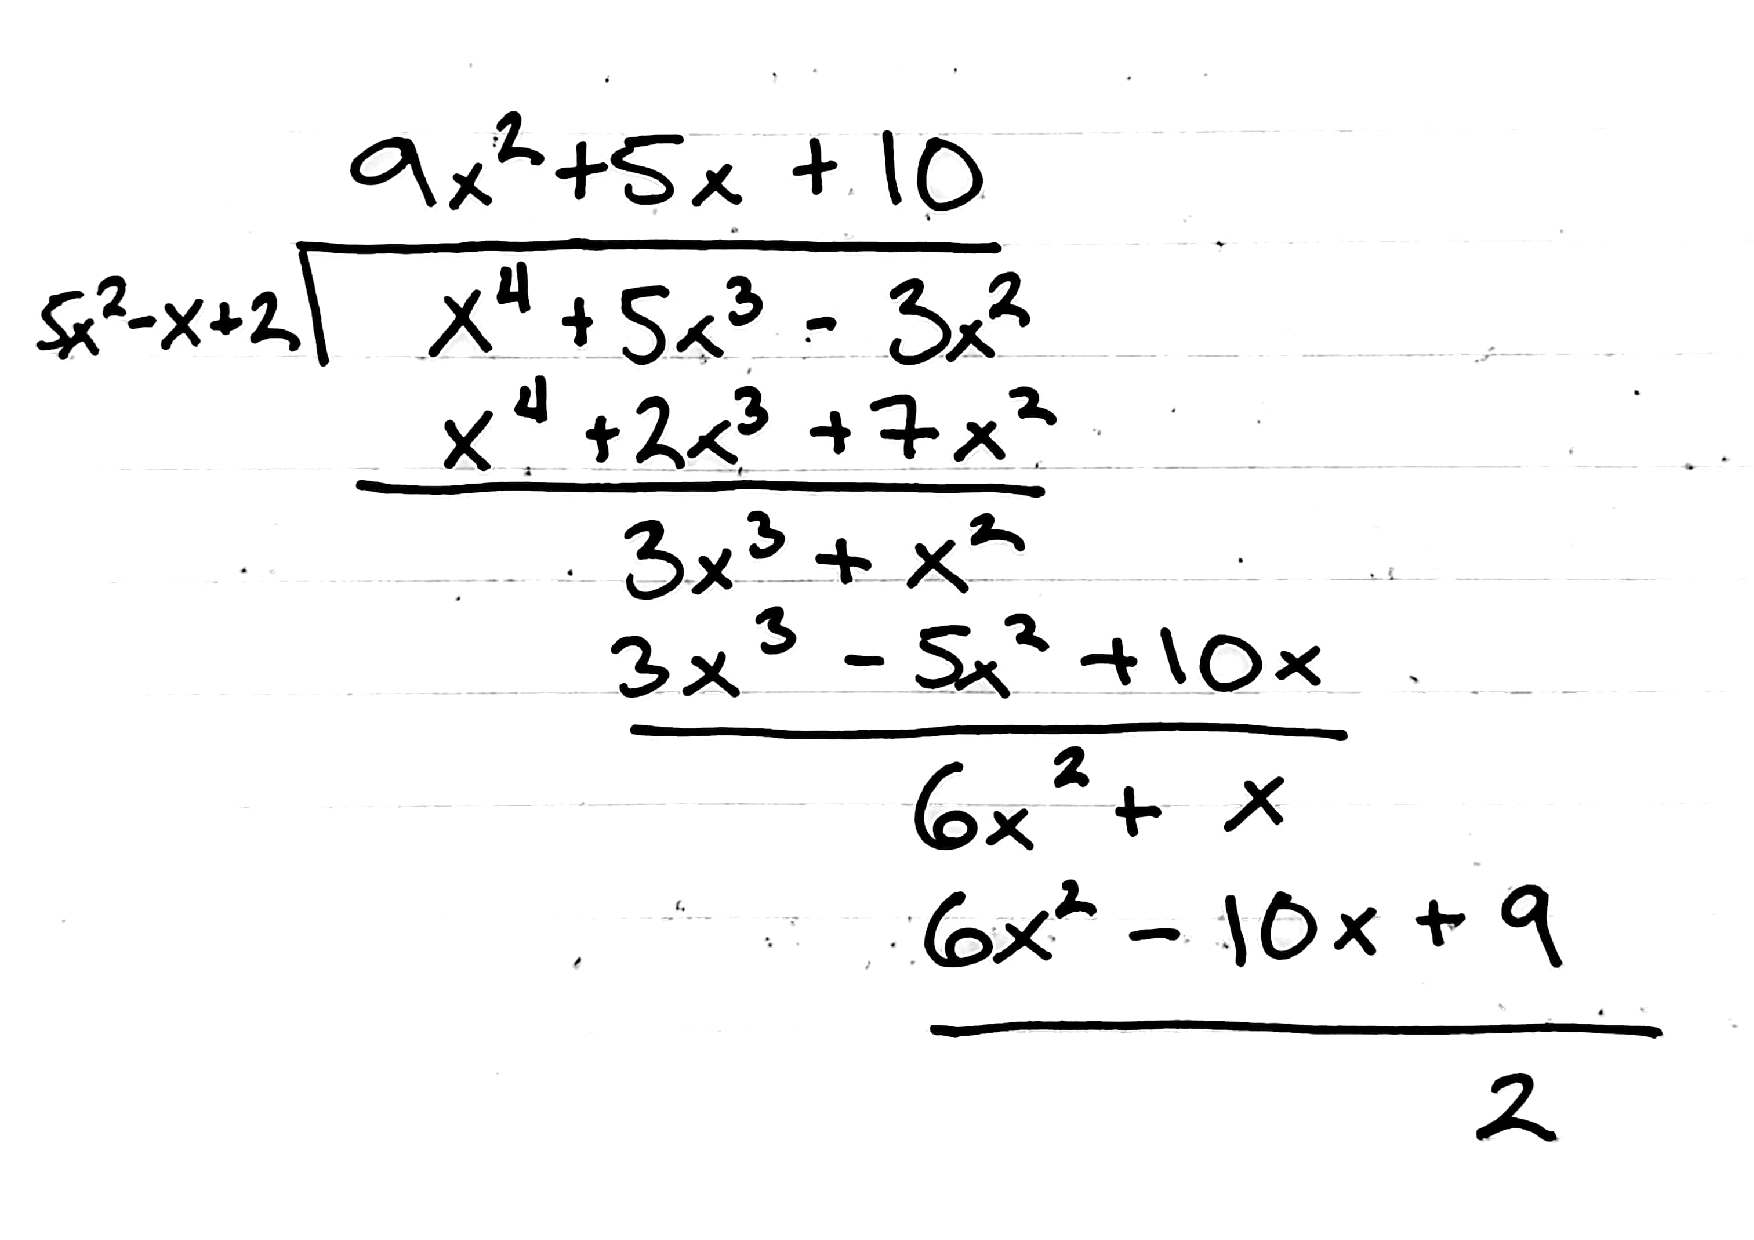
\includegraphics[page=1,width=0.6\textwidth]{longdiv.pdf}
\end{figure}

Therefore $q(x) = 9x^2 + 5x + 10$ and $r(x) = 2$.

\subsection*{23.10}
Note that $-1$ is a zero, meaning the linear factor $x+1$ is in its factorization. The division algorithm using $x+1$ as the divisor gives $x^2 + x + 1$ which by inspection factors into $(x-2)(x-4)$. Therefore the factorization is
\[
    (x+1)(x-2)(x-4)
.\]

\subsection*{23.14}
Using $p = 2$ it follows that the polynomial satisfies the Einstein criterion meaning it is irreducible over $\Q$. The quadratic formula gives the zeros
\[
    \frac{-8 \pm \sqrt{64 + 8}}{2} = -4 \pm 6\sqrt{2}
\]
which are both real and therefore it is not irreducible over $\R$. The fundamental theorem of algebra implies every polynomial in $\C$ is not irreducible.

\subsection*{23.16}
If $f$ factors in $\Q$, then it has a zero in $\Q$. Since $a_0 = -8 \neq 0$, it must therefore have a zero in $\Z$ that divides $-8$. This means the possible candidates are $x = \pm 1, \pm 2, \pm 4, \pm 8$. However, none of the candidates are zero's, meaning there isn't a zero in $\Z$ and hence it must be irreducible in $\Q$.

\subsection*{23.20}
Choosing $p = 3$ gives
\[
    1x^{10} + 0x^3 + 0x - 0
.\]
Therefore it satisfies the Einstein criterion.

\subsection*{23.30}
An irreducible polynomial will need to have a non zero constant term, otherwise $0$ would be a zero of the polynomial. Since $f(x)$ is zero iff $2 f(x)$ is zero, this means that the set of irreducible polynomials with leading coefficient $1$ give rise to the other irreducible polynomials, their doubles. The only cases (coefficients are expressed as ordered tuples for space) of this then are 
\begin{align*}
    &(1, 0, 2, 1), (2, 0, 1, 2) \\
    &(1, 0, 2, 2), (2, 0, 1, 1) \\
    &(1, 1, 0, 2), (2, 2, 0, 1) \\
    &(1, 2, 0, 1), (2, 1, 0, 2) \\
    &(1, 1, 1, 2), (2, 2, 2, 1) \\
    &(1, 1, 2, 1), (2, 2, 1, 2) \\
    &(1, 2, 1, 1), (2, 1, 2, 2) \\
    &(1, 2, 2, 2), (2, 1, 1, 1)
\end{align*}
Therefore there are 16 irreducible cubics in $\Z_3[x]$

\subsection*{23.34}
\begin{proof}
    Let $p$ be prime and consider $x^p + a$ where $a \in \Z_p$. Since $-a$ is less than $p$ and not divided by $p$, then by Fermat's Little Theorem,
    \[
        (-a)^{p-1} \equiv 1 \pmod{p} \implies (-a)^{p} + a \equiv 0 \pmod{p}
    .\]
    Therefore $x = -a$ is a zero of $x^p + a$ meaning it is not irreducible.
\end{proof}

\subsection*{23.36}
\begin{proof}
    By the division algorithm,
    \[
        f(x) = g(x)(x-\alpha) + c
    \]
    for some constant $c \in F$. Applying the evaluation homomorphism at $\alpha$ gives
    \[
        \phi_{\alpha}(f(x)) = g(\alpha)(\alpha - \alpha) + c = g(\alpha) \cdot 0 + c = c
    .\]
    Therefore the remainder is $f(\alpha)$.
\end{proof}

\subsection*{23.37}
\begin{@empty}
\newcommand{\homo}[1][m]{\conj{\sigma_{#1}}}

\subsubsection*{Part A}
\begin{proof}
    Note that $\homo$ is linear and multiplicative over elements of $\Z$. Let $f(x) = \sum_{i=0}^\infty a_i x^i$ and $g(x) = \sum_{j=0}^\infty b_j x^j$ be elements of $\Z[x]$. Checking if $\homo$ is an additive group homomorphism gives
    \begin{align*}
        \homo(f(x) + g(x)) &= \homo\qty(\sum_{i=0}^\infty a_i x^i + \sum_{j=0}^\infty b_j x^j) \\
                           &= \homo\qty(\sum_{i=0}^\infty (a_i + b_i) x^i) \\
                           &= \sum_{i=0}^\infty \homo(a_i + b_i) x^i \\
                           &= \sum_{i=0}^\infty \homo(a_i) x^i + \homo(b_i) x^i \\
                           &= \homo(f(x)) + \homo(g(x))
    \end{align*}
    Checking if $\homo$ is multiplicative gives
    \begin{align*}
        \homo(f(x) g(x)) &= \homo\qty(\sum_{i=0}^\infty \qty(\sum_{j=0}^i a_j b_{i-j}) x^i) \\
        &= \sum_{i=0}^\infty \qty(\sum_{j=0}^i \homo(a_j b_{i-j})) x^i \\
        &= \sum_{i=0}^\infty \qty(\sum_{j=0}^i \homo(a_j) \homo(b_{i-j})) x^i \\
        &= \homo(f(x)) \homo(g(x))
    .\end{align*}
    Therefore $\homo$ is a ring homomorphism from $\Z[x]$ to $\Z_{m}[x]$
\end{proof}

\subsubsection*{Part B}
\begin{proof}
    Assume towards contradiction that that some $f(x)$ factors into two polynomials of degree $r,s < \deg f$ and $\homo(f(x))$ has degree $n$ but is irreducible. Since $\homo$ is a ring homomorphism and $f(x) = g(x) h(x)$ with $\deg h, \deg g < n$, it follows
    \[
        \homo(f(x)) = \homo(g(x) h(x)) =  \homo(g(x)) \homo(h(x))
    .\]
    However, this gives a factorization of $\homo(f(x))$ into polynomials with degree smaller than $n$, a contradiction.
\end{proof}

\subsubsection*{Part C}
Taking $m = 5$ gives $\homo[5](x^3 + 17x + 36) = x^3 + 2x + 1$. Inspection shows that $x = 0, 1, -1, 2, -2$ aren't zeroes and therefore the polynomial is irreducible in $\Z[x]$ by the previous part. Since it is irreducible in $\Z[x]$, it is irreducible in $\Q[x]$.
    
\end{@empty}

\end{document}
